This appendix collects implementation details that support reproducibility but would otherwise interrupt the flow of the main text.

\subsection{Feature Blocks and Practical Implementation}

The final predictor design is organized into persistence, technical, macro-financial, and multiscale blocks. The persistence block contains current volatility, 5-day average volatility, and 22-day average volatility. The technical block contains close-to-close returns, intraday returns, overnight gaps, ATR, RSI, MACD, and short-window stress summaries. The macro-financial block contains index-specific implied-volatility proxies together with rates, term spreads, financial conditions, recession information, and, in the expanded setting, credit spreads, policy uncertainty, and volatility-term-structure variables. The multiscale block contains causal wavelet summaries extracted from the target volatility proxy, absolute returns, and implied-volatility series.

\begin{table}[H]
\caption{Key implementation choices used in the final reproducible pipeline. Each setting is fixed before the final out-of-sample evaluation.}
\label{tab:implementation_choices}
\centering
\small
\setlength{\tabcolsep}{4pt}
\renewcommand{\arraystretch}{1.12}
\begin{tabular}{>{\raggedright\arraybackslash}p{0.23\textwidth}>{\raggedright\arraybackslash}p{0.20\textwidth}>{\raggedright\arraybackslash}p{0.49\textwidth}}
\toprule
Component & Final choice & Practical rationale \\
\midrule
Core sample & SPX, NDQ, and DJI daily panels & Balances market representativeness, data length, and replication cost \\
Main volatility proxy & Rogers--Satchell & Uses OHLC information while remaining stable under a public daily-data design \\
Robustness target & Parkinson & Tests whether conclusions depend on the main OHLC proxy \\
Wavelet basis and depth & Symlet-4, \(J=3\) & Produces a compact short/medium/long decomposition without over-expanding the feature space \\
Wavelet extraction window & Minimum 128 and maximum 256 observations & Preserves causal computation while avoiding excessive edge instability \\
Rolling estimation window & 1260 trading days & Approximates a five-year learning window for stable walk-forward estimation \\
Refit frequency & Every 5 trading days & Controls runtime while keeping model updates frequent enough for daily deployment \\
Warning threshold & Rolling 90th percentile of future volatility & Adapts to cross-index scale differences and regime shifts \\
Decision threshold & \(F_2\)-optimal cutoff & Prioritizes recall because missed high-risk episodes are more costly than false alarms \\
Primary evaluation metric & QLIKE & Appropriate for positive volatility forecasts and imperfect volatility proxies \\
\bottomrule
\end{tabular}
\end{table}


\subsection{Rolling Evaluation Details}

Every rolling split follows the same sequence: construct all features from the trailing estimation window, estimate the horizon-specific regression model, apply the QLIKE-oriented calibration floor, compute the rolling high-risk threshold, estimate the warning model, and then score the next out-of-sample observation. No preprocessing step is fitted on the full sample. This includes scaling, clipping, wavelet extraction, calibration-floor estimation, and warning-threshold selection.

\subsection{Notation, Metrics, and Testing Notes}

The notation table in the main text is intentionally compact. In implementation terms, the most important distinction is between raw predictors, multiscale summaries, and post-calibration forecasts. Raw predictors are observable market and macro-financial variables. Multiscale summaries are deterministic transformations of causal windows of these variables. Post-calibration forecasts are the quantities actually sent to the QLIKE evaluator and the warning layer. This distinction matters because only the final step changes the loss geometry without changing the underlying training target.

The evaluation metrics also answer different questions. QLIKE emphasizes scale-sensitive volatility calibration, RMSE and MAE measure point error magnitude, PR-AUC measures event ranking under class imbalance, and Brier score evaluates probability calibration. DM tests speak to realized loss differences, whereas CW tests speak to incremental predictive content in nested settings. The article reports both because neither on its own is sufficient to characterize the contribution of a public-data hybrid model.

\subsection{Additional Robustness Interpretation}

The main robustness exercises serve different purposes. The expanded public risk-data experiment tests whether the proposed multiscale design benefits from richer external predictors that remain publicly accessible. The Parkinson experiment tests whether the main conclusion depends on a specific OHLC volatility proxy. Together, these extensions indicate that the proposed framework should be interpreted as a public-data integration pipeline rather than a single narrowly optimized model.

\subsection{Additional Architecture and Diagnostic Figures}

Figure~\ref{fig:encoder_fusion_heads_appendix} provides the module-level expansion of the main architecture used in Section~\ref{sec:methodology}. Figures~\ref{fig:forecast_panels_appendix}, \ref{fig:multiscale_signal_heatmap_appendix}, and~\ref{fig:block_contribution_heatmap_appendix} report secondary diagnostics that support, but do not define, the main computational claims in Section~\ref{sec:results}.

\begin{figure}[!t]
\centering
\includegraphics[width=0.96\textwidth]{figures/structure.png}
\caption{Module-level expansion of the CMWSL pipeline architecture. The figure details the four sequential layers described in Section~\ref{sec:methodology}: the HAR persistence block, the causal stationary-wavelet-transform multiscale layer with scale-wise summary statistics, the cross-index spillover layer, and the horizon-specific forecast and warning heads. The mapping from raw features to final predictions is fully causal and deterministic given the rolling window.}
\label{fig:encoder_fusion_heads_appendix}
\end{figure}

\begin{figure}[!t]
\centering
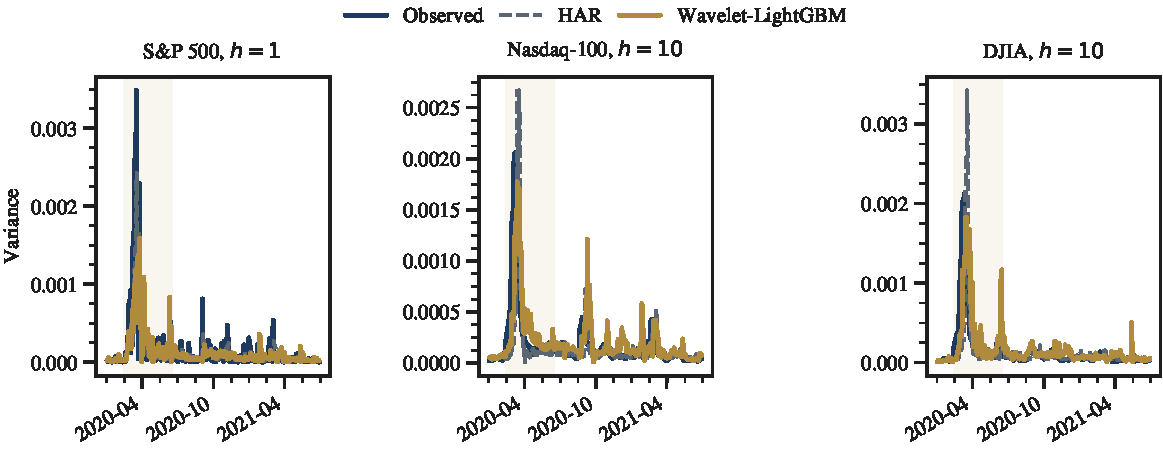
\includegraphics[width=0.94\textwidth]{figures/fig05_forecast_panels.pdf}
\caption{Representative out-of-sample forecast traces in the main and expanded-data specifications. The wavelet-enhanced model follows the build-up and decay of stress episodes more smoothly at \(h=5\) and \(h=10\), whereas isolated daily spikes still tend to favour the parsimonious HAR benchmark.}
\label{fig:forecast_panels_appendix}
\end{figure}

\begin{figure}[!t]
\centering
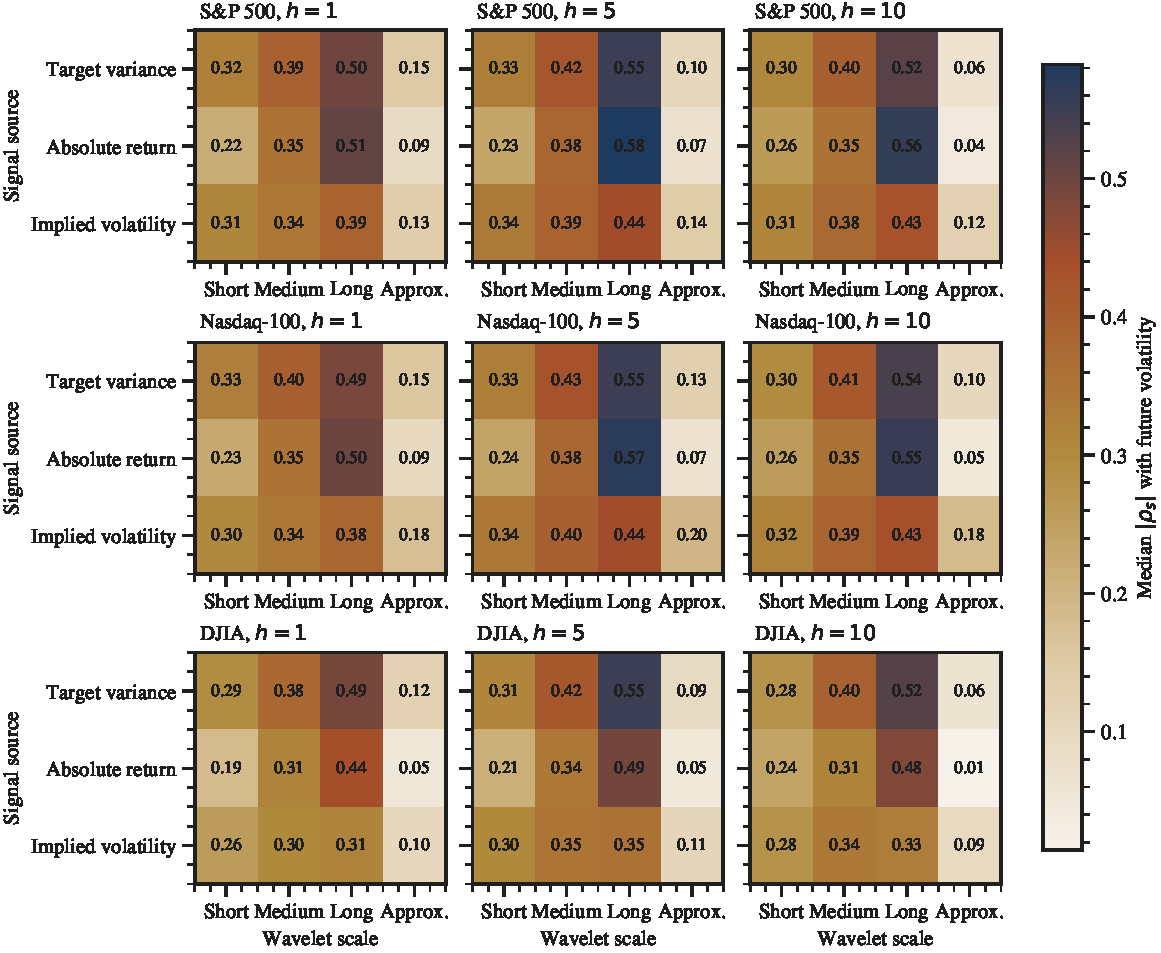
\includegraphics[width=0.94\textwidth]{figures/fig11_multiscale_signal_heatmap.pdf}
\caption{Multiscale signal map in the expanded public risk-data panel. Each cell reports the median absolute Spearman association between a wavelet feature group and future volatility.}
\label{fig:multiscale_signal_heatmap_appendix}
\end{figure}

\begin{figure}[!t]
\centering
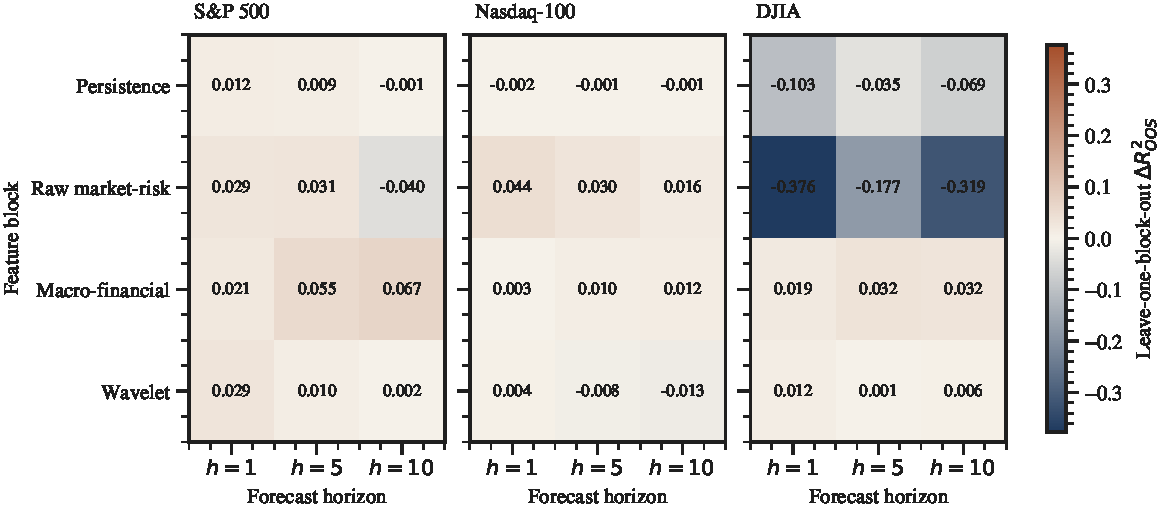
\includegraphics[width=0.94\textwidth]{figures/fig12_block_contribution_heatmap.pdf}
\caption{Surrogate leave-one-block-out contribution map in the expanded public risk-data panel. Each cell reports the change in out-of-sample \(R^2\) from removing one feature block from a fixed train/test surrogate regression on block embeddings.}
\label{fig:block_contribution_heatmap_appendix}
\end{figure}

\begin{figure}[!t]
\centering
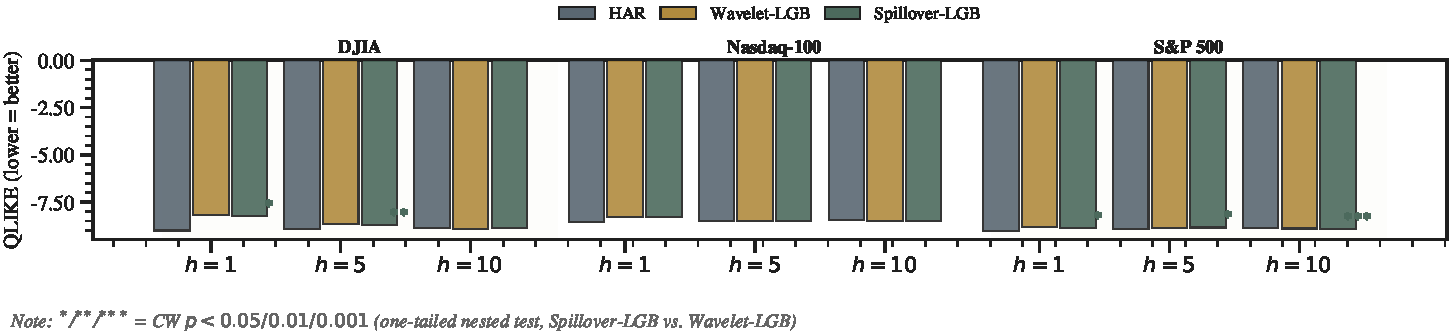
\includegraphics[width=0.94\textwidth]{figures/fig_spillover_qlike_bars.pdf}
\caption{QLIKE comparison across indices and forecast horizons for the three models in the spillover ablation. Asterisks above the Spillover-LGB bar indicate Clark--West significance at the corresponding cell.}
\label{fig:spillover_qlike_bars_appendix}
\end{figure}

\begin{figure}[!t]
\centering
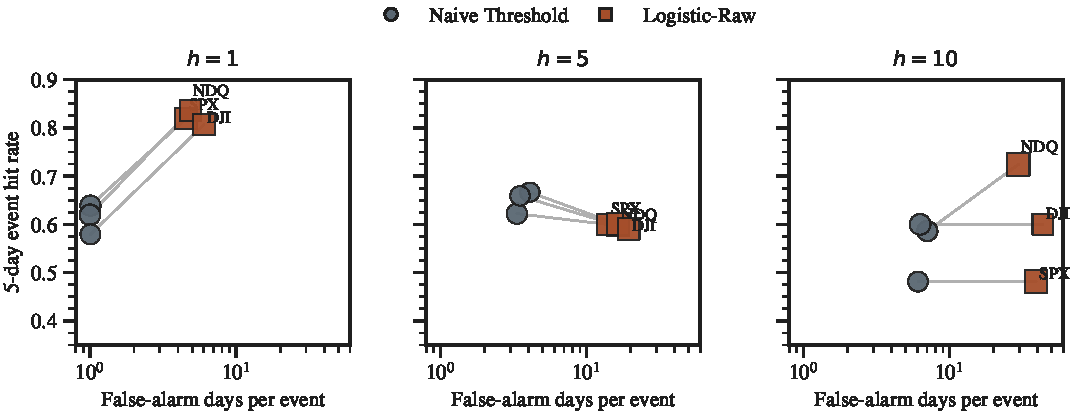
\includegraphics[width=0.96\textwidth]{figures/fig14_warning_event_frontier.pdf}
\caption{Event-based warning frontier at the index--horizon level. The horizontal axis reports false-alarm days per event on a log scale, the vertical axis reports the five-day event hit rate, and marker size scales with the mean lead time. Grey line segments connect the two warning rules within the same index--horizon cell.}
\label{fig:warning_event_frontier_appendix}
\end{figure}

\subsection{Additional Statistical Tables}

\begin{table}[!t]
\caption{Forecast comparison tests against HAR in the main specification.}
\label{tab:significance_tests}
\centering
\scriptsize
\setlength{\tabcolsep}{3.5pt}
\resizebox{\textwidth}{!}{%
\begin{tabular}{lllllll}
\toprule
Index & Horizon & Model & DM stat & DM p-value & CW stat & CW p-value \\
\midrule
DJIA & 1 & LightGBM & 3.572 & 0.0004 & 2.060 & 0.0197 \\
DJIA & 1 & Wavelet-LightGBM & 3.344 & 0.0008 & 2.440 & 0.0073 \\
DJIA & 5 & LightGBM & 1.925 & 0.0542 & 2.333 & 0.0098 \\
DJIA & 5 & Wavelet-LightGBM & 1.458 & 0.1448 & 2.503 & 0.0062 \\
DJIA & 10 & LightGBM & -0.228 & 0.8194 & 2.901 & 0.0019 \\
DJIA & 10 & Wavelet-LightGBM & -1.158 & 0.2467 & 2.983 & 0.0014 \\
Nasdaq-100 & 1 & LightGBM & 2.927 & 0.0034 & 2.935 & 0.0017 \\
Nasdaq-100 & 1 & Wavelet-LightGBM & 3.967 & 0.0001 & 3.542 & 0.0002 \\
Nasdaq-100 & 5 & LightGBM & -0.990 & 0.3224 & 4.516 & 0.0000 \\
Nasdaq-100 & 5 & Wavelet-LightGBM & -0.353 & 0.7239 & 4.927 & 0.0000 \\
Nasdaq-100 & 10 & LightGBM & -1.080 & 0.2801 & 4.682 & 0.0000 \\
Nasdaq-100 & 10 & Wavelet-LightGBM & -2.145 & 0.0320 & 4.821 & 0.0000 \\
S\&P 500 & 1 & LightGBM & 2.639 & 0.0083 & 2.641 & 0.0041 \\
S\&P 500 & 1 & Wavelet-LightGBM & 2.614 & 0.0090 & 2.669 & 0.0038 \\
S\&P 500 & 5 & LightGBM & 1.004 & 0.3155 & 2.489 & 0.0064 \\
S\&P 500 & 5 & Wavelet-LightGBM & 0.900 & 0.3683 & 2.678 & 0.0037 \\
S\&P 500 & 10 & LightGBM & -0.180 & 0.8572 & 2.784 & 0.0027 \\
S\&P 500 & 10 & Wavelet-LightGBM & 0.202 & 0.8398 & 2.736 & 0.0031 \\
\bottomrule
\end{tabular}
}
\end{table}


\begin{table}[!t]
\caption{Broad-market regime-conditioned spillover gains. Entries report $\Delta$QLIKE = Spillover-LGB minus Wavelet-LGB for DJIA and S\&P 500 pooled observations. Negative values indicate that cross-index spillover features improve accuracy.}
\label{tab:spillover_regime}
\centering
\small
\setlength{\tabcolsep}{5.0pt}
\renewcommand{\arraystretch}{1.10}
\begin{tabular}{lccc}
\toprule
Regime & $h=1$ & $h=5$ & $h=10$ \\
\midrule
Bottom 20\% VIX & -0.042 & 0.009 & -0.004 \\
COVID 2020--2021 & -0.377 & 0.122 & 0.011 \\
Expansion & -0.054 & -0.016 & \best{-0.006} \\
Post-2022 & -0.028 & -0.109 & -0.002 \\
Recession & \best{-0.674} & \best{-0.361} & 0.145 \\
Top 20\% VIX & -0.069 & -0.045 & -0.002 \\
\bottomrule
\end{tabular}
\end{table}


\subsection{Project Assets}

The core manuscript results are generated from three merged result packages: the main Rogers--Satchell specification, the expanded public risk-data specification, and the Parkinson specification. The manuscript figures and tables are produced from these merged packages through deterministic scripts stored in the project repository. This setup is intended to make the final article easy to audit, rerun, and extend.
